\documentclass[aspectratio=169,10pt]{beamer}
\usepackage[utf8]{inputenc}
\usepackage[T1]{fontenc}
\usepackage[french]{babel}
\usepackage{graphicx}
\usepackage{booktabs}
\usepackage{tabularx}

\definecolor{navy}{HTML}{12304A}
\definecolor{teal}{HTML}{087E83}
\definecolor{gold}{HTML}{D49A22}
\definecolor{pale}{HTML}{EFF5F7}
\definecolor{muted}{HTML}{5B6B78}
\usetheme{Madrid}
\setbeamertemplate{navigation symbols}{}
\setbeamertemplate{headline}{}
\setbeamercolor{structure}{fg=teal}
\setbeamercolor{palette primary}{bg=navy,fg=white}
\setbeamercolor{palette secondary}{bg=teal,fg=white}
\setbeamercolor{frametitle}{bg=white,fg=navy}
\setbeamercolor{block title}{bg=teal,fg=white}
\setbeamercolor{block body}{bg=pale,fg=navy}
\setbeamercolor{alerted text}{fg=gold}
\setbeamerfont{frametitle}{series=\bfseries}
\setbeamersize{text margin left=0.55cm,text margin right=0.55cm}
\setbeamertemplate{frametitle}{%
  \nointerlineskip
  \begin{beamercolorbox}[wd=\paperwidth,ht=5.5ex,dp=1.2ex]{frametitle}
    \makebox[\paperwidth]{%
      \makebox[1.8cm][c]{
\includegraphics[height=0.4in]{images/logoUAC1.png}}%
      \makebox[\dimexpr\paperwidth-3.6cm\relax][c]{\insertframetitle}%
      \makebox[1.8cm][c]{
\includegraphics[height=0.4in]{images/logoIfri.png}}%
    }
  \end{beamercolorbox}
  {\color{teal}\hrule height 0.8pt}
}
\setbeamertemplate{footline}{%
  \leavevmode\hbox{%
    \begin{beamercolorbox}[wd=.78\paperwidth,ht=2.5ex,dp=1ex,leftskip=1em]{author in head/foot}
      \color{white}\insertshorttitle
    \end{beamercolorbox}%
    \begin{beamercolorbox}[wd=.22\paperwidth,ht=2.5ex,dp=1ex,center]{date in head/foot}
      \color{white}\insertframenumber{} / \inserttotalframenumber
    \end{beamercolorbox}%
  }
}
\newcommand{\shot}[2]{%
  \begin{minipage}[t]{\linewidth}\centering
    \includegraphics[width=\linewidth,height=1.18in,keepaspectratio]{images/C3/#1.png}\par
    \vspace{0.15em}{\scriptsize\color{muted}#2}
  \end{minipage}%
}
\newcommand{\platformshot}[2]{%
  \begin{minipage}[t]{\linewidth}\centering
    \includegraphics[width=\linewidth,height=1.18in,keepaspectratio]{#1}\par
    \vspace{0.15em}{\scriptsize\color{muted}#2}
  \end{minipage}%
}
\title[Assistant juridique béninois]{Conception et implémentation d'un assistant conversationnel intelligent pour la compréhension du Code du Numérique en République du Bénin}
\author{Yélian Joanès Domicov \textbf{AZON}}
\institute{Licence en Informatique — Génie Logiciel\\IFRI — Université d'Abomey-Calavi}
\date{Année académique 2026--2027}

\begin{document}

\begin{frame}[plain]
  \noindent\makebox[\textwidth][s]{
\includegraphics[height=1.05cm]{images/logoUAC1.png}\hfill
\includegraphics[height=0.8cm]{images/logoIfri.png}}
  \vspace{0.2cm}
  \begin{center}
    {\color{navy}\LARGE\bfseries
      Conception et implémentation d'un assistant\\
      conversationnel intelligent\\
      pour la compréhension du Code du Numérique\\
      en République du Bénin\par}
    \vspace{0.15cm}{\color{gold}\rule{0.24\textwidth}{1.4pt}\par}
    \vspace{0.1cm}{\large Présentation du mémoire de fin de cycle\par}
  \end{center}
  \vfill
  \begin{center}
    {\large Yélian Joanès Domicov \textbf{AZON}\par}
    \vspace{0.15cm}{\normalsize Encadrant : Armand \textbf{ACCROMBESSI}\par}
    \vspace{0.1cm}{\small Licence en Informatique — Génie Logiciel\\IFRI — Université d'Abomey-Calavi\\2026--2027\par}
  \end{center}
\end{frame}

\begin{frame}{Plan de la présentation}
  \begin{itemize}
    \setlength{\itemsep}{0.9em}
    \large\bfseries
    \item Introduction
    \item 1 — Revue de littérature et étude de plateformes existantes
    \item 2 — Analyse, conception et choix techniques
    \item 3 — Présentation, évaluations et perspectives
    \item Conclusion
  \end{itemize}
\end{frame}

\section{Introduction}
\begin{frame}{Contexte et problématique}
  \begin{block}{Un accès au droit encore difficile}
    Le Code du Numérique béninois couvre les communications électroniques, les données personnelles, le commerce électronique et la cybercriminalité. Sa longueur et son vocabulaire technique compliquent la recherche d'une disposition précise.
  \end{block}
  \begin{columns}[T,onlytextwidth]
    \begin{column}{.31\textwidth}\begin{block}{Corpus volumineux}Plus de 600 articles répartis en livres, titres et chapitres.\end{block}\end{column}
    \begin{column}{.31\textwidth}\begin{block}{Textes modifiés}La Loi N° 2020-35 modifie la Loi N° 2017-20 : une version ancienne peut induire en erreur.\end{block}\end{column}
    \begin{column}{.31\textwidth}\begin{block}{Risque juridique}Une réponse plausible mais erronée ou non sourcée fragilise la confiance.\end{block}\end{column}
  \end{columns}
  \vspace{0.2cm}\centering\textbf{Problématique :} comment interroger simplement le Code et obtenir une réponse explicable, vérifiable et reliée à ses articles ?
\end{frame}

\begin{frame}{Objectifs et contribution}
  \begin{columns}[T,onlytextwidth]
    \begin{column}{.48\textwidth}
      \begin{block}{Objectif général}
        Concevoir un assistant conversationnel fondé sur le RAG pour répondre de façon fiable et sourcée aux questions relatives au Code du Numérique béninois.
      \end{block}
      \begin{block}{Objectifs spécifiques}
        \begin{itemize}\setlength\itemsep{0.3em}
          \item Consolider et structurer le corpus juridique.
          \item Retrouver les articles par question ou référence.
          \item Développer une interface simple et accessible.
          \item Sécuriser et tester l'API et les comptes.
        \end{itemize}
      \end{block}
    \end{column}
    \begin{column}{.48\textwidth}
      \begin{block}{Livrables du projet}
        \begin{itemize}\setlength\itemsep{0.4em}
          \item Explorateur du Code et assistant conversationnel.
          \item Recherche hybride et génération contrainte par les sources.
          \item Gestion des comptes, conversations et signalements.
          \item Outils d'administration et évaluation du système.
        \end{itemize}
      \end{block}
      \centering\large\color{teal}\textbf{Un accès plus simple, une réponse traçable.}
    \end{column}
  \end{columns}
\end{frame}

\section{1. Revue de littérature}
\begin{frame}{Fondements conceptuels et cadre juridique}
  \begin{columns}[T,onlytextwidth]
    \begin{column}{.48\textwidth}
      \begin{block}{Notions mobilisées}
        \begin{itemize}\setlength\itemsep{0.35em}
          \item Un agent conversationnel permet l'interrogation en langage naturel.
          \item Un LLM formule des réponses, mais peut produire des hallucinations.
          \item Le RAG récupère des passages documentaires avant la génération.
          \item Embeddings et reranking améliorent la recherche et le classement.
        \end{itemize}
      \end{block}
    \end{column}
    \begin{column}{.48\textwidth}
      \begin{block}{Corpus juridique ciblé}
        \begin{itemize}\setlength\itemsep{0.35em}
          \item Code du Numérique : Loi N\textsuperscript{o} 2017-20, modifiée par la Loi N\textsuperscript{o} 2020-35.
          \item Sept livres couvrant notamment les communications électroniques, les données personnelles, le commerce électronique et la cybersécurité.
          \item Corpus consolidé décrit dans le mémoire : 629 articles.
        \end{itemize}
      \end{block}
    \end{column}
  \end{columns}
  \begin{alertblock}{Enjeu de la revue}
    La recherche documentaire réduit le risque d'hallucination, mais la fiabilité dépend aussi de la qualité, de l'actualité et de la structuration du corpus.
  \end{alertblock}
\end{frame}

\begin{frame}{Solutions existantes : juridiques et professionnelles}
  \begin{columns}[T,onlytextwidth]
    \begin{column}{.48\textwidth}\platformshot{images/C1/LawPavillon.jpg}{LawPavilion — recherche juridique professionnelle, Nigeria}\end{column}
    \begin{column}{.48\textwidth}\platformshot{images/C1/Timi.jpg}{TIMI AI — assistant juridique, Nigeria}\end{column}
  \end{columns}
  \begin{block}{Autres références étudiées}
    Jurisprudence.cc (espace OHADA), Juribot, JuridiqueIA et AideJuridique.ai. Ces outils diffèrent par leur juridiction, leur public cible et leur périmètre documentaire.
  \end{block}
\end{frame}

\begin{frame}{Assistants citoyens et positionnement du projet}
  \begin{columns}[T,onlytextwidth]
    \begin{column}{.32\textwidth}\platformshot{images/C1/Wakili CRM.jpg}{Wakili.org — assistance juridique citoyenne, Kenya}\end{column}
    \begin{column}{.32\textwidth}\platformshot{images/C1/JusticePadi.png}{JusticePadi — assistance juridique citoyenne, Nigeria}\end{column}
    \begin{column}{.32\textwidth}\platformshot{images/C1/EMY1.png}{EMY 101 — assistant administratif, Côte d'Ivoire}\end{column}
  \end{columns}
  \begin{alertblock}{Besoin ciblé au Bénin}
    GPT BJ facilite le dialogue sur des textes béninois. Le mémoire identifie un besoin complémentaire : un assistant dédié au Code du Numérique consolidé, avec des réponses sourcées à l'article et vérifiables.
  \end{alertblock}
  \centering\small La comparaison fait ressortir le positionnement du projet : corpus juridique ciblé, références explicites et fonctionnalités testables.
\end{frame}

\section{2. Analyse, conception et choix techniques}
\begin{frame}{Architecture logicielle et choix techniques}
  \begin{columns}[T,onlytextwidth]
    \begin{column}{.21\textwidth}\begin{block}{Interface}\centering Next.js 14\\React 18\\Tailwind CSS\\\small Parcours web, explorateur, chat\end{block}\end{column}
    \begin{column}{.04\textwidth}\centering\vspace{1.2cm}{\large\color{gold}$\rightarrow$}\end{column}
    \begin{column}{.21\textwidth}\begin{block}{API métier}\centering FastAPI\\Python / Pydantic\\JWT + RBAC\\\small Authentification et orchestration\end{block}\end{column}
    \begin{column}{.04\textwidth}\centering\vspace{1.2cm}{\large\color{gold}$\rightarrow$}\end{column}
    \begin{column}{.21\textwidth}\begin{block}{Persistance}\centering PostgreSQL\\Neon.tech\\SQLAlchemy\\\small Comptes, échanges, métriques\end{block}\end{column}
    \begin{column}{.04\textwidth}\centering\vspace{1.2cm}{\large\color{gold}$\rightarrow$}\end{column}
    \begin{column}{.16\textwidth}\begin{block}{IA locale}\centering Pipeline RAG\\Ollama\\Gemma 3 (1B)\end{block}\end{column}
  \end{columns}
  \vspace{0.35cm}
  \begin{block}{Sécurité et déploiement}
    Mots de passe hachés avec bcrypt, jetons JWT, contrôle d'accès par rôle, suppression en cascade ; frontend web, API conteneurisée et base de données managée.
  \end{block}
\end{frame}

\begin{frame}[plain]
  \centering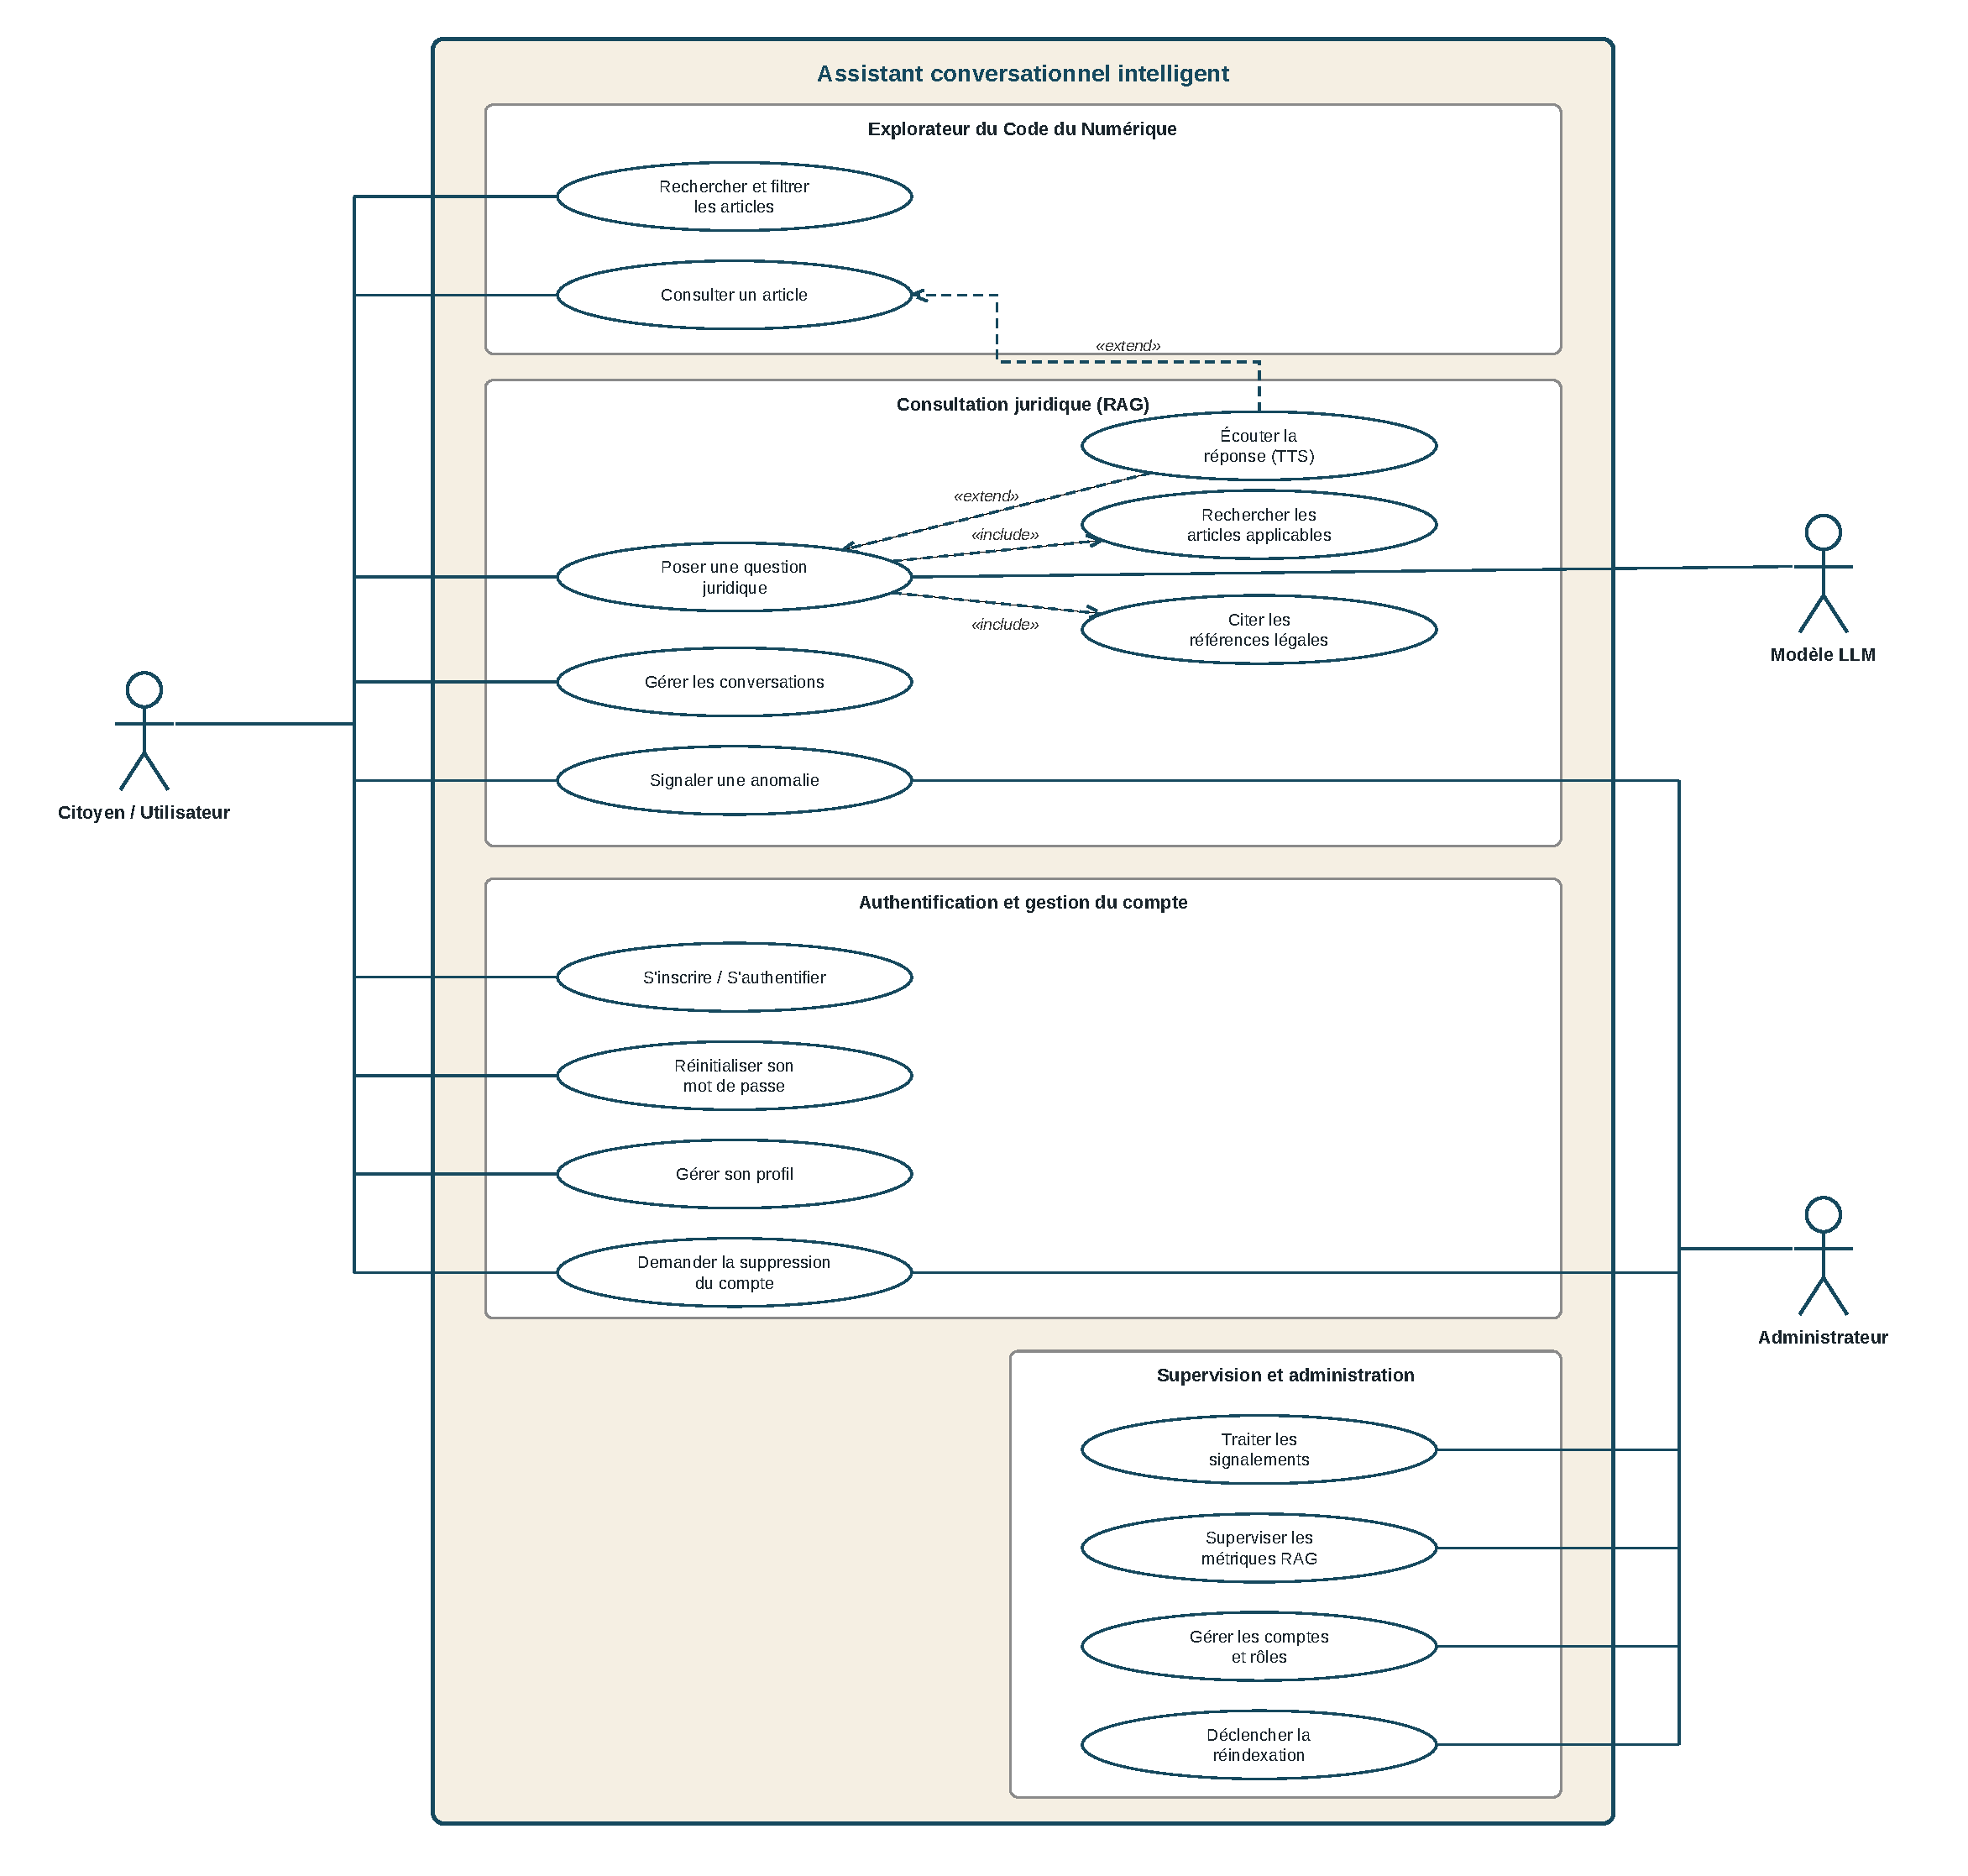
\includegraphics[width=.96\paperwidth,height=.9\paperheight,keepaspectratio]{images/C2/DCU.pdf}
\end{frame}

\begin{frame}{Diagramme de classes : structure des données}
  \centering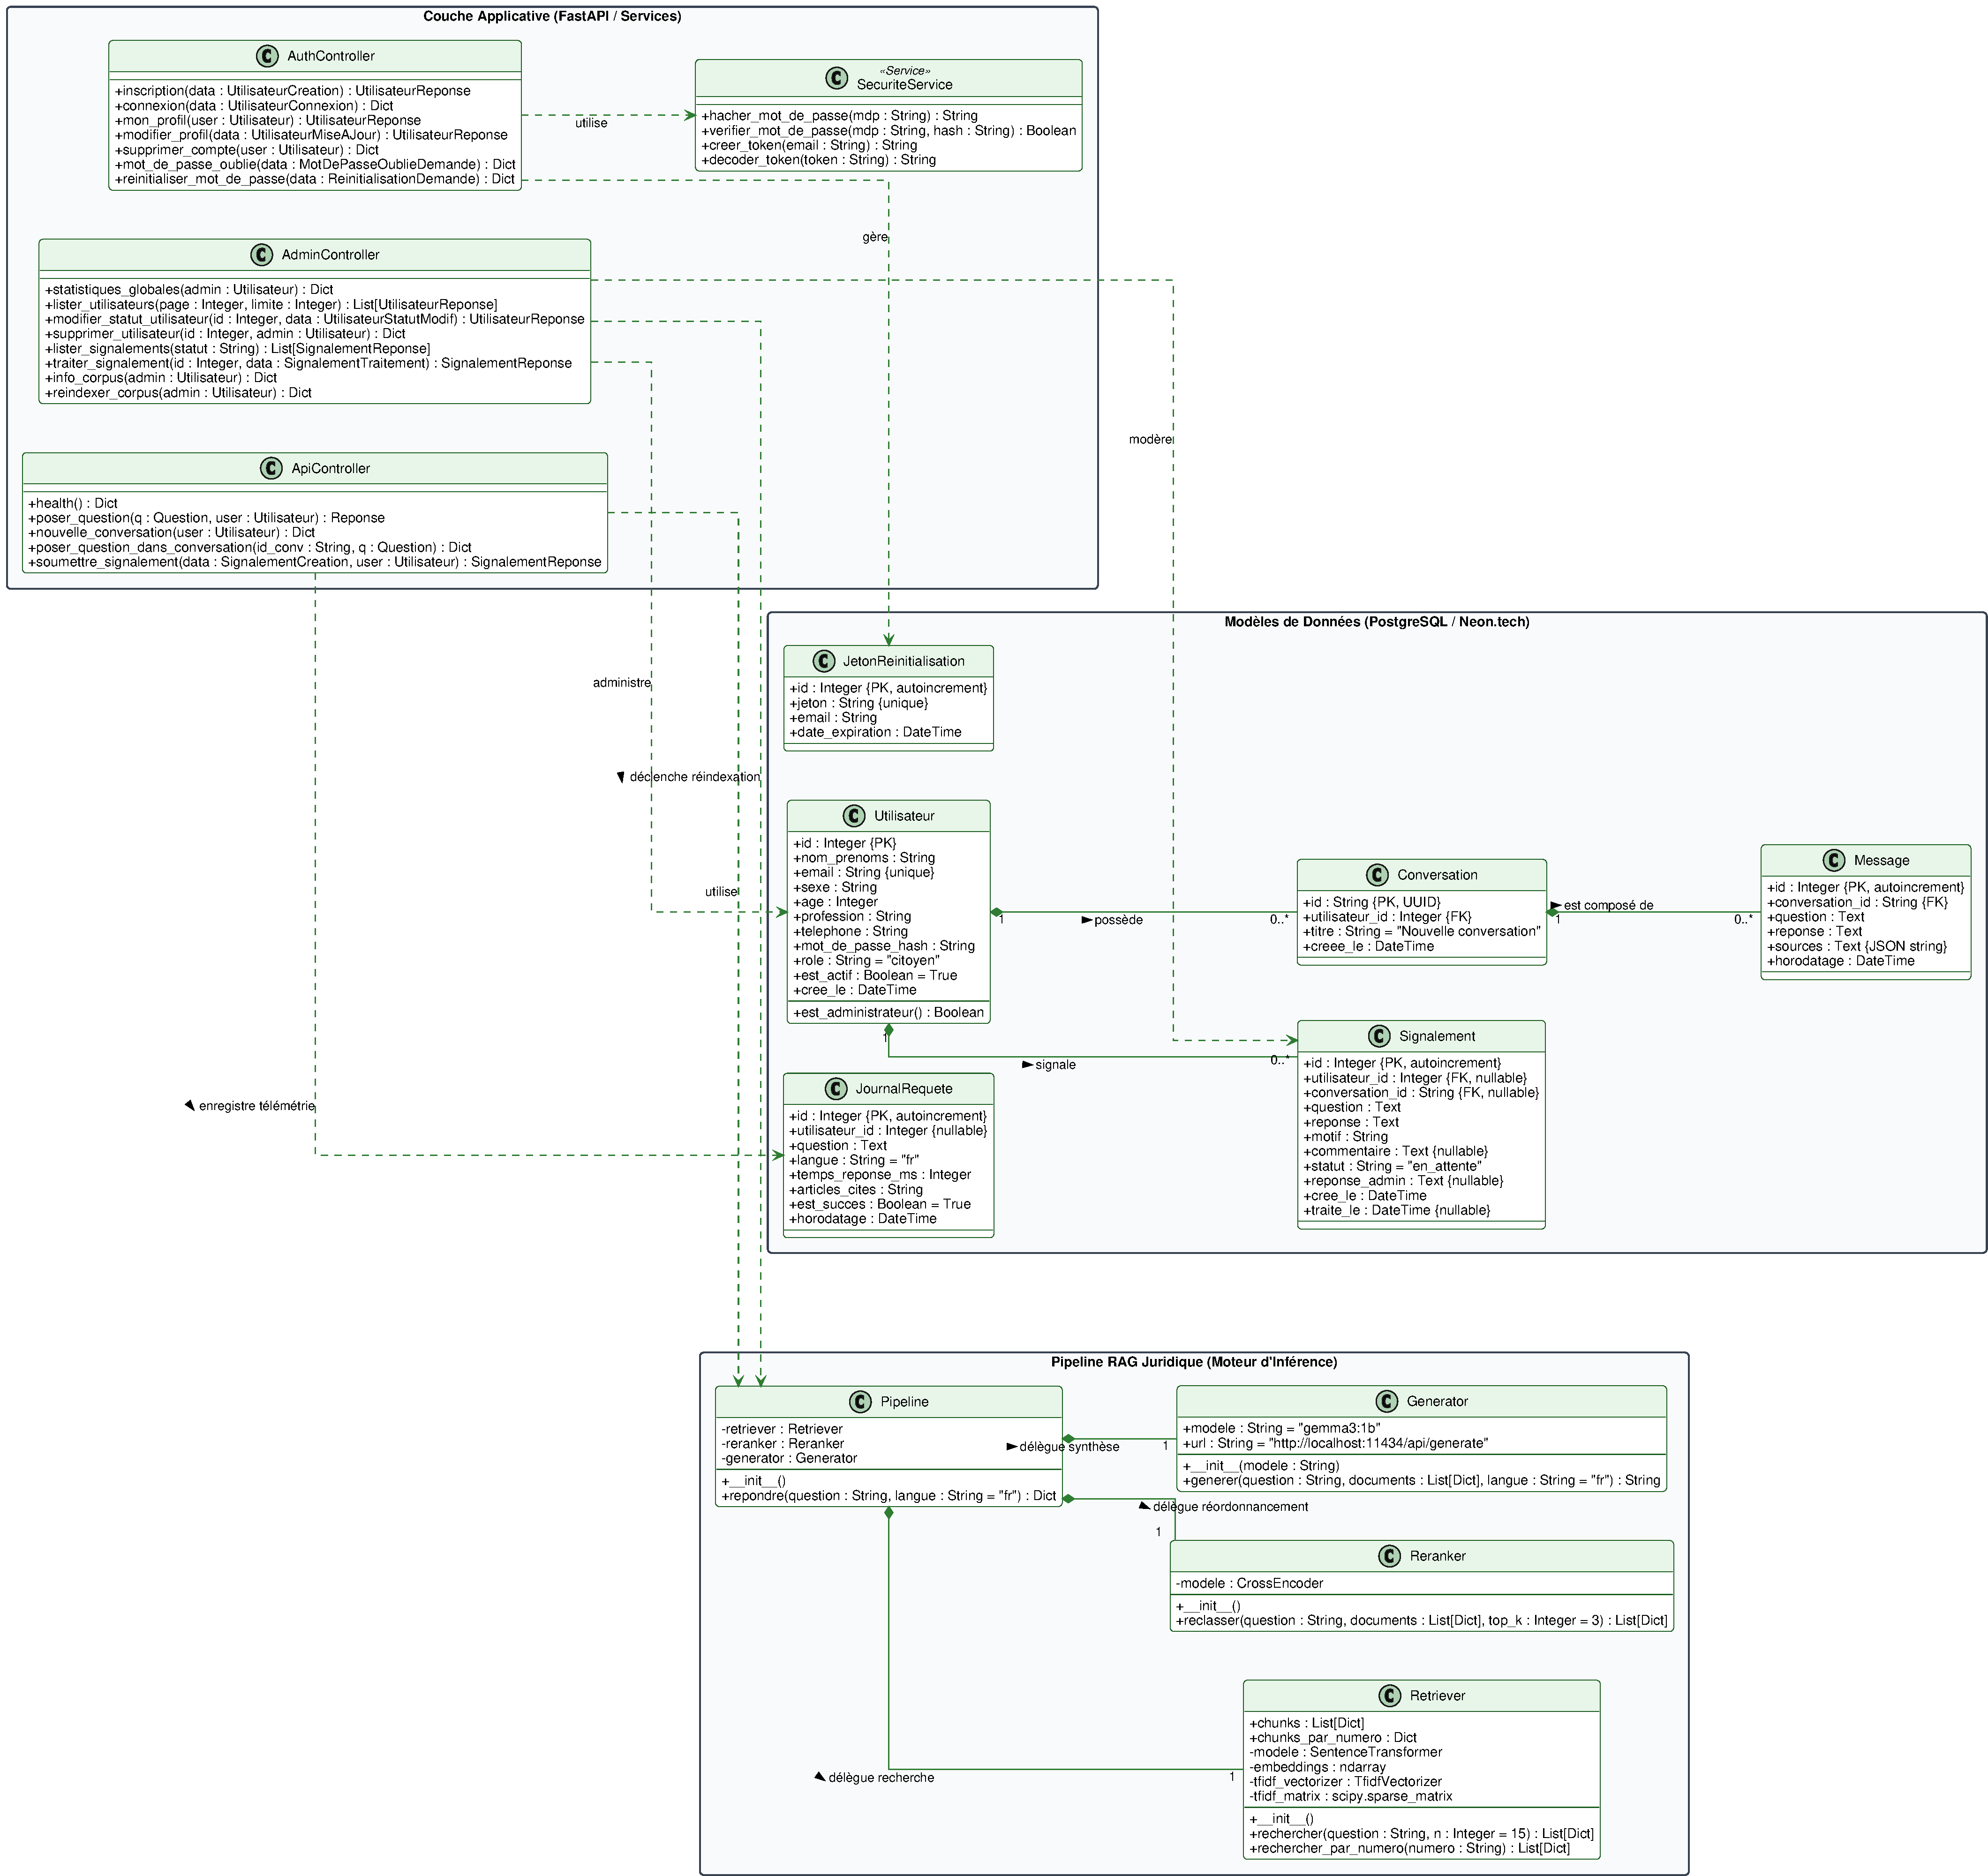
\includegraphics[width=.94\textwidth,height=.74\textheight,keepaspectratio]{images/C2/DC.pdf}
  \vspace{0.1cm}\par\scriptsize Utilisateur, Conversation, Message, Article, ChunkDocumentaire et services associés.
\end{frame}

\begin{frame}{Diagramme de séquence : consultation juridique}
  \centering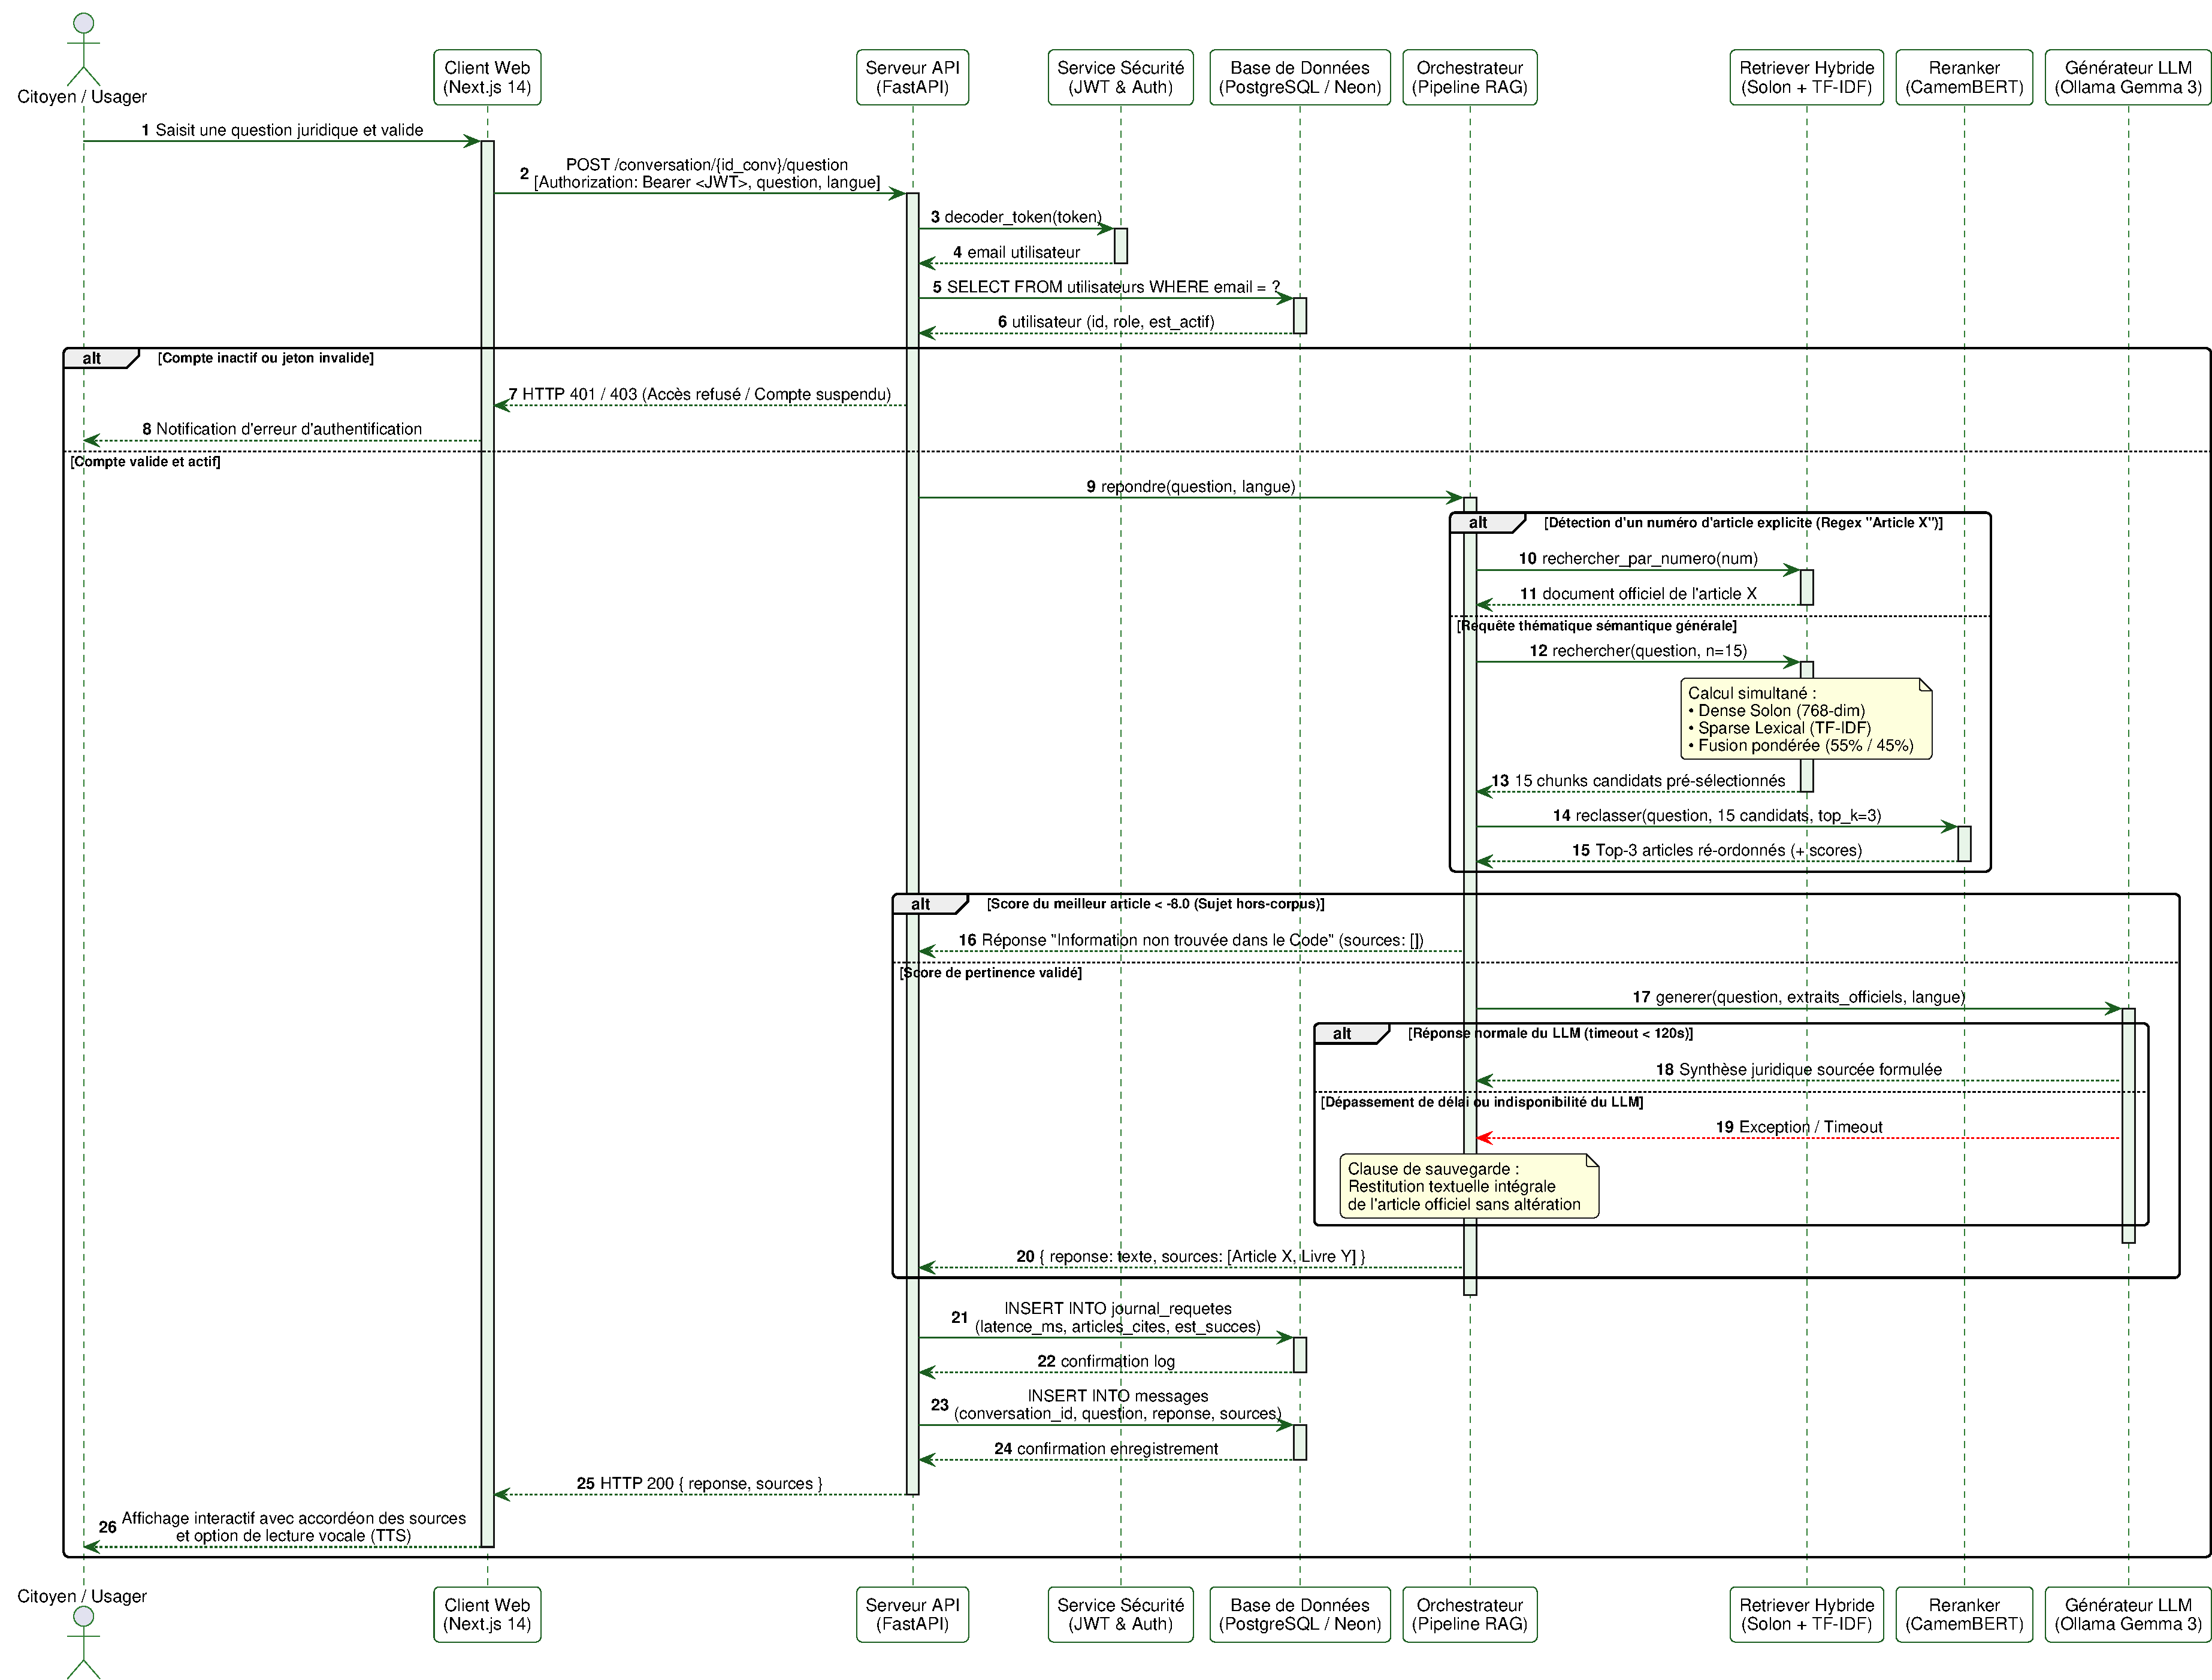
\includegraphics[width=.98\textwidth,height=.74\textheight,keepaspectratio]{images/C2/DS.pdf}
  \vspace{0.1cm}\par\scriptsize Authentification, recherche, reranking, génération ou repli, persistance et restitution.
\end{frame}

\begin{frame}{Diagramme d'activités : déroulement du traitement}
  \begin{columns}[T,onlytextwidth]
    \begin{column}{.48\textwidth}\centering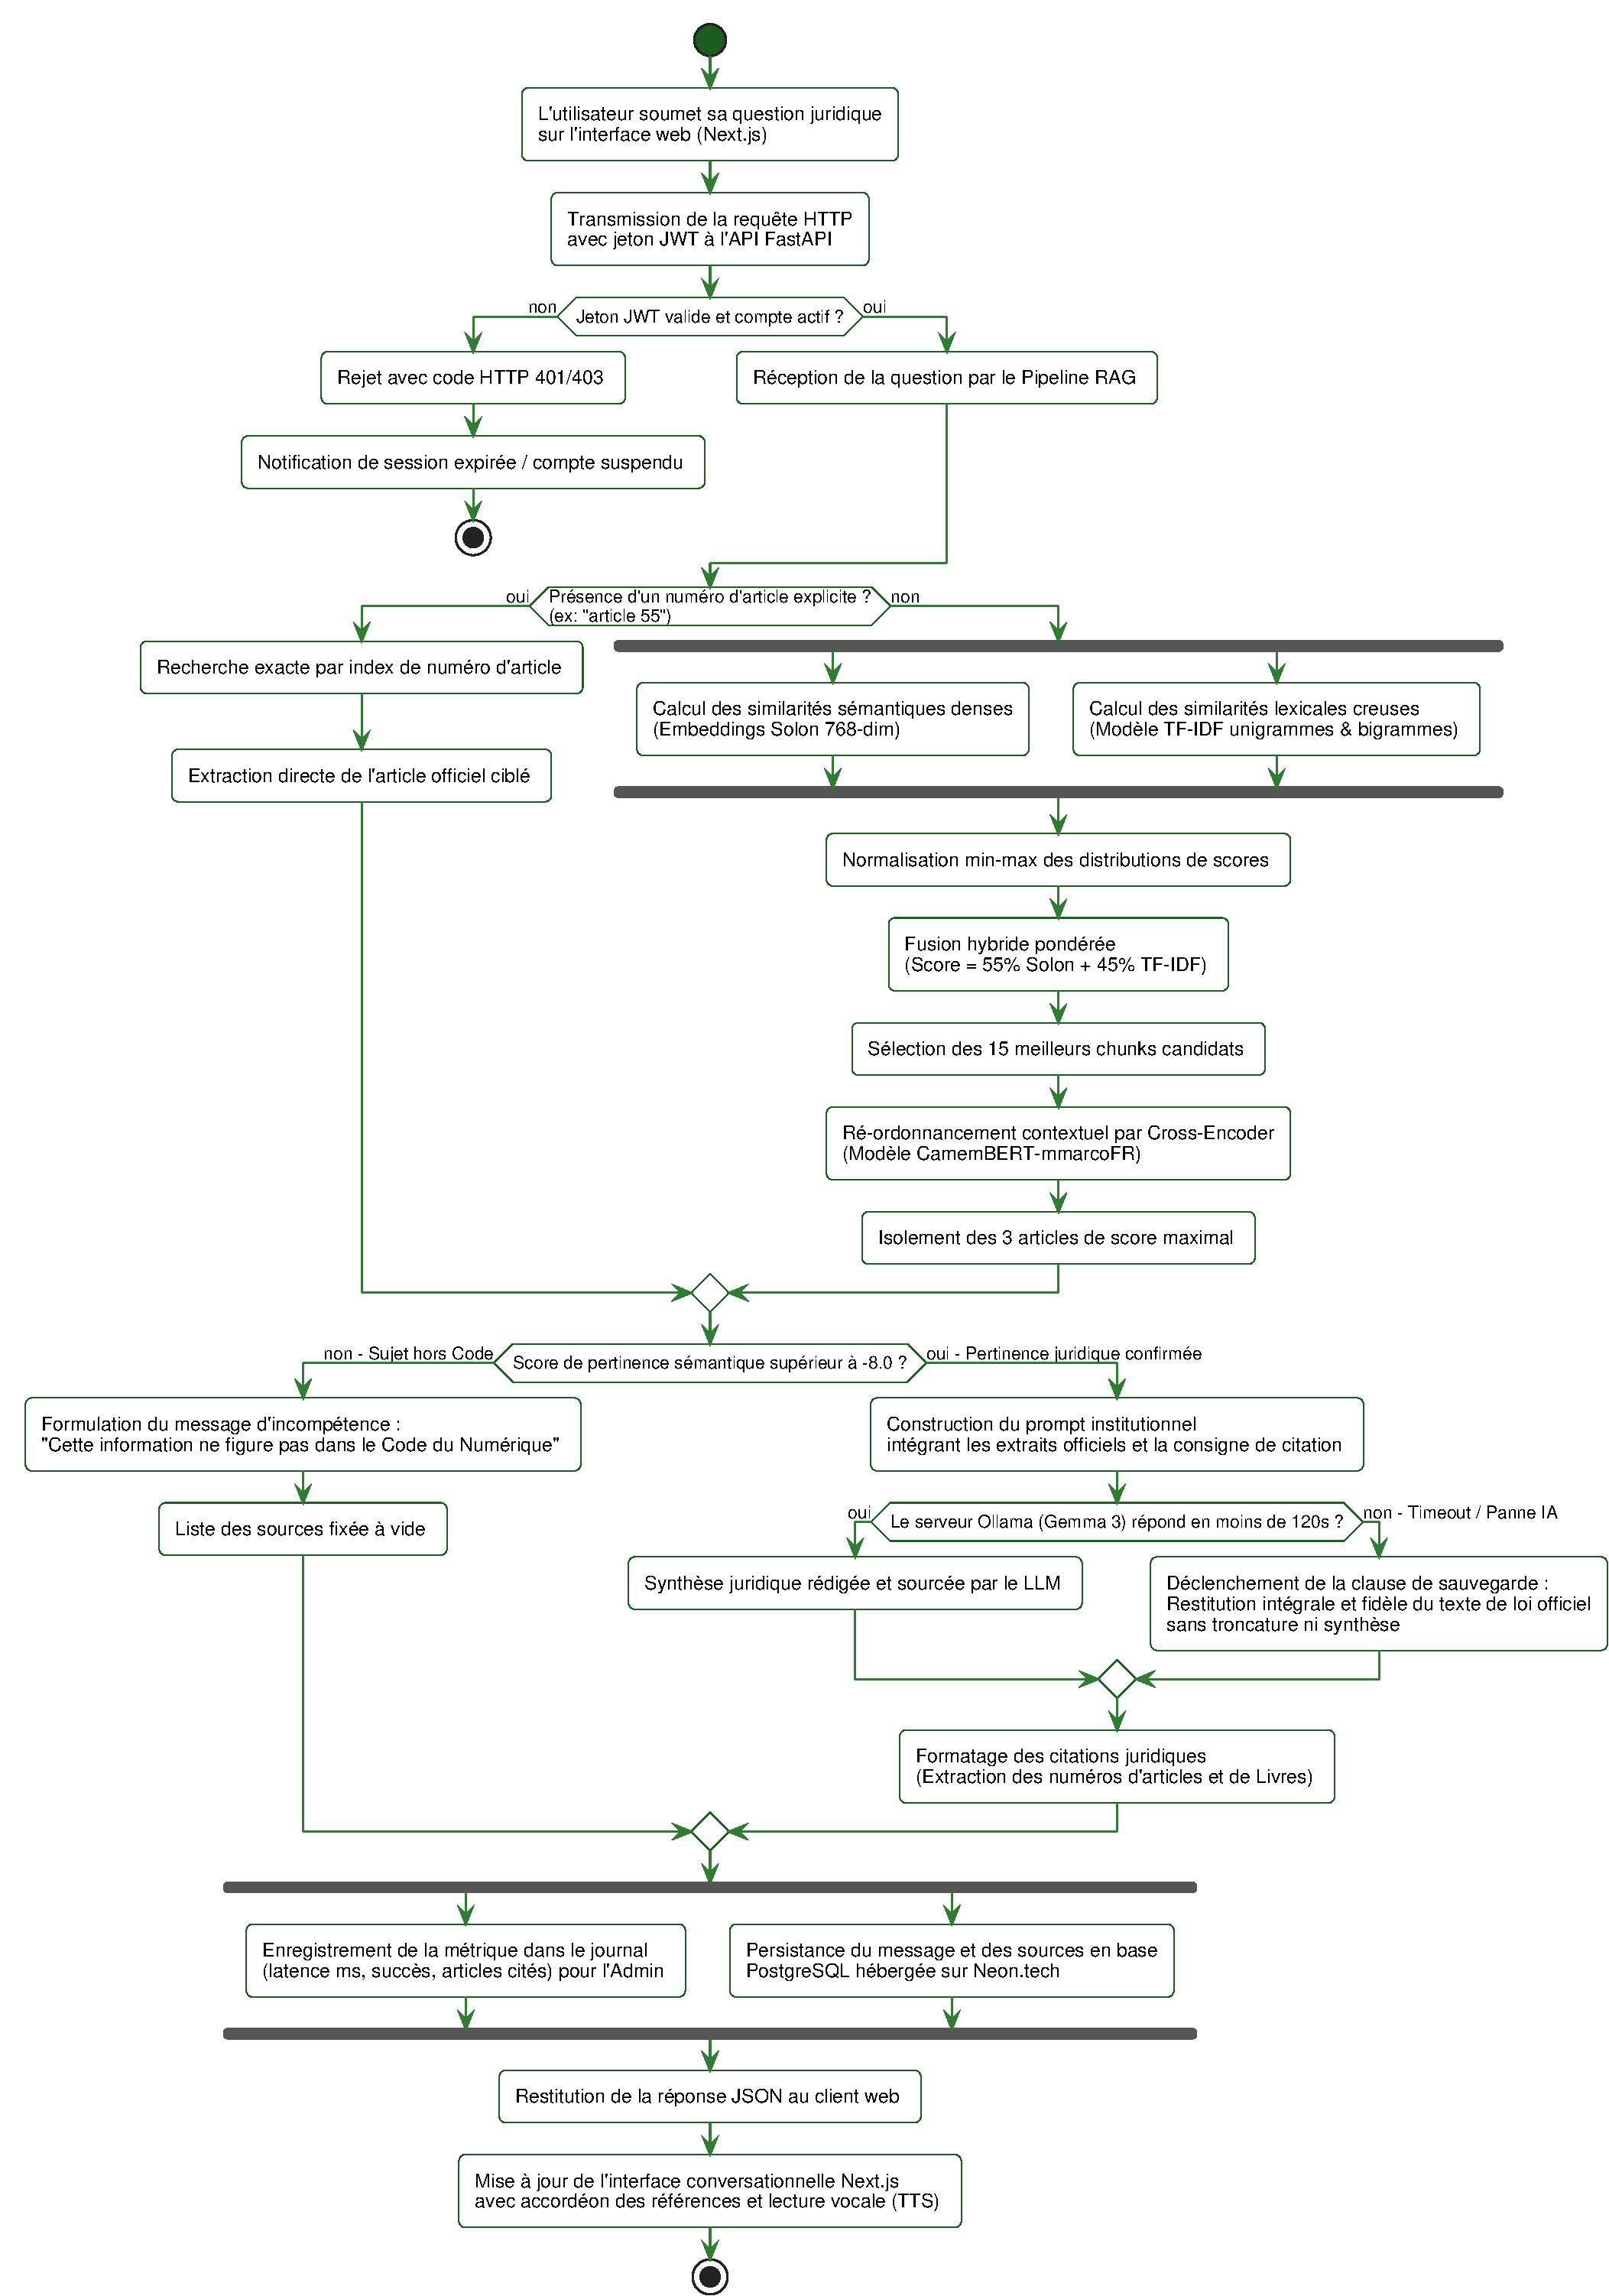
\includegraphics[width=\linewidth,height=.74\textheight,keepaspectratio]{images/C2/DA.pdf}\end{column}
    \begin{column}{.48\textwidth}
      \begin{block}{Étapes du flux}
        \begin{enumerate}\setlength\itemsep{0.45em}
          \item Vérifier la requête et l'identité.
          \item Choisir la recherche directe ou hybride.
          \item Réordonner les articles candidats.
          \item Générer, refuser ou activer le repli.
          \item Enregistrer réponse et métriques.
        \end{enumerate}
      \end{block}
    \end{column}
  \end{columns}
\end{frame}

\begin{frame}[plain]
  \centering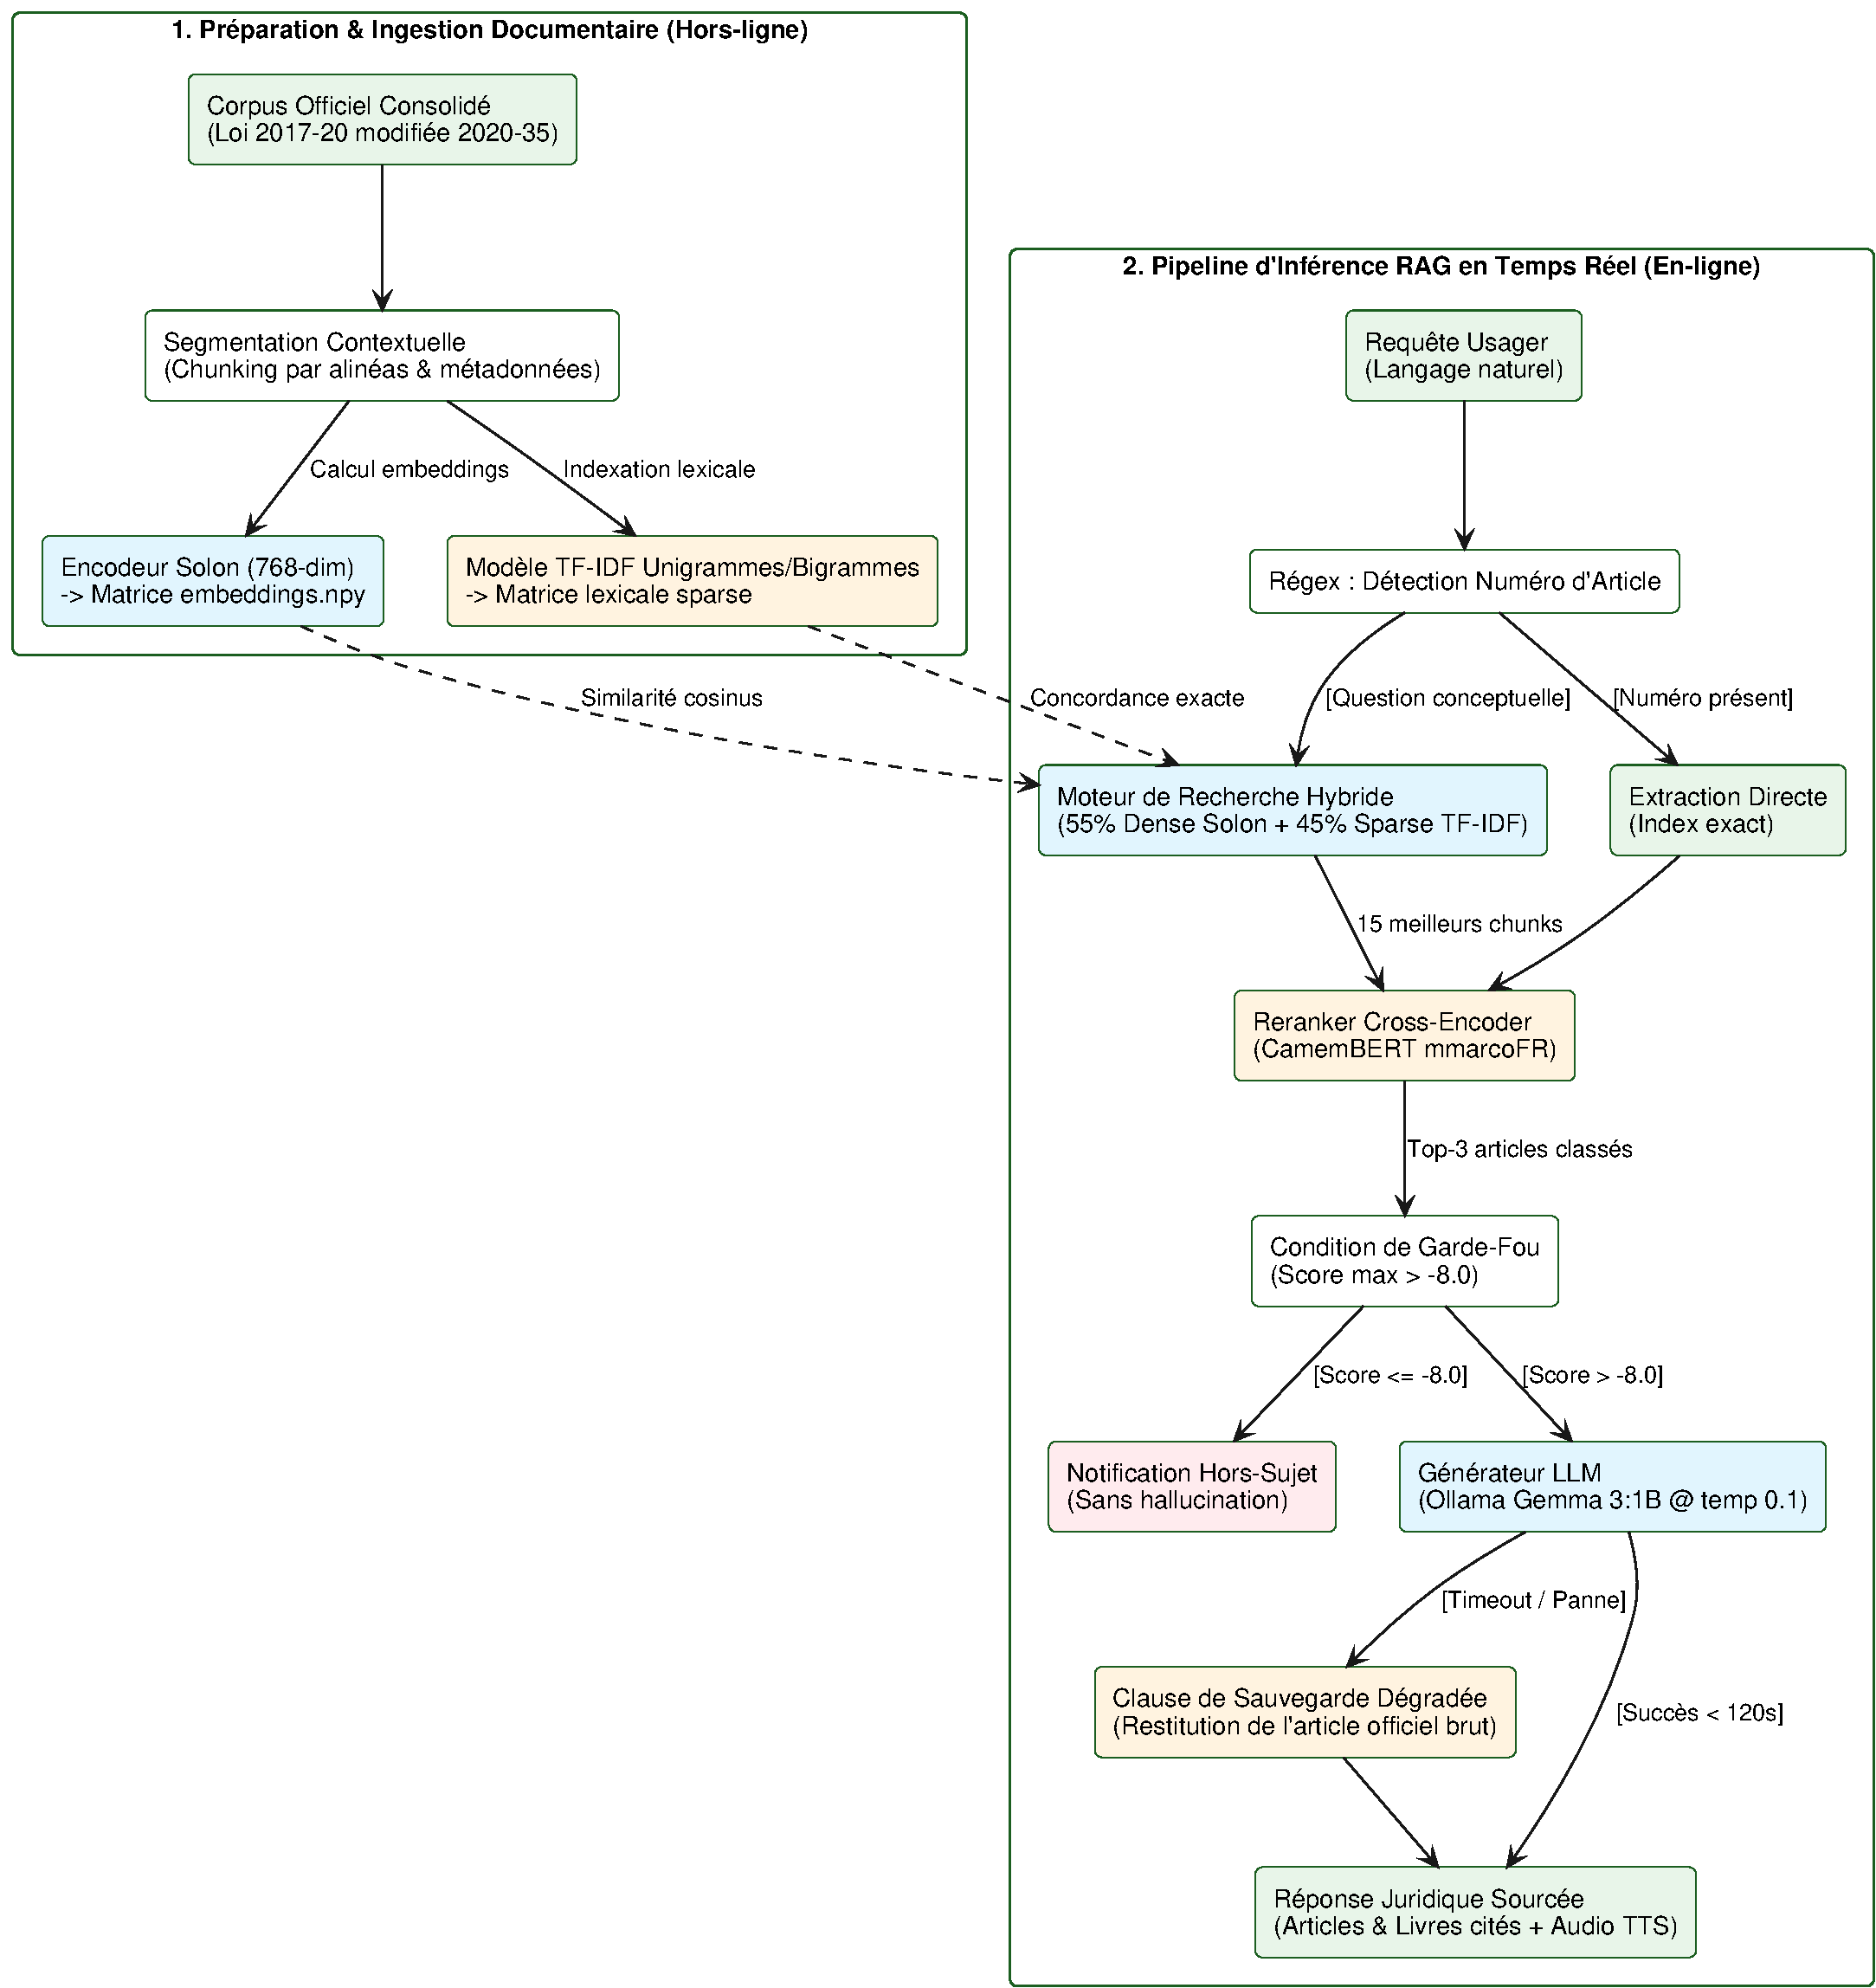
\includegraphics[width=.92\paperwidth,height=.91\paperheight,keepaspectratio]{images/C2/Pipeline_RAG.pdf}
\end{frame}

\begin{frame}{Pipeline RAG : de la question à la réponse}
  \begin{columns}[T,onlytextwidth]
    \begin{column}{.18\textwidth}\begin{block}{1. Corpus}\small Texte consolidé, articles et métadonnées.\end{block}\end{column}
    \begin{column}{.04\textwidth}\centering\vspace{1cm}{\large\color{gold}$\rightarrow$}\end{column}
    \begin{column}{.2\textwidth}\begin{block}{2. Recherche}\small Article direct ou recherche dense Solon + lexicale TF--IDF.\end{block}\end{column}
    \begin{column}{.04\textwidth}\centering\vspace{1cm}{\large\color{gold}$\rightarrow$}\end{column}
    \begin{column}{.2\textwidth}\begin{block}{3. Classement}\small Fusion pondérée, 15 candidats, cross-encoder CamemBERT.\end{block}\end{column}
    \begin{column}{.04\textwidth}\centering\vspace{1cm}{\large\color{gold}$\rightarrow$}\end{column}
    \begin{column}{.2\textwidth}\begin{block}{4. Réponse}\small Gemma 3 avec Ollama ; réponse sourcée, refus ou repli.\end{block}\end{column}
  \end{columns}
  \vspace{0.35cm}
  \begin{alertblock}{Recherche hybride}
    Solon : embeddings juridiques denses de 768 dimensions. TF--IDF : correspondance lexicale. Fusion après normalisation : 55\% sémantique / 45\% lexicale ; CamemBERT retient les 2 à 3 articles les plus pertinents.
  \end{alertblock}
\end{frame}

\begin{frame}{Garde-fous : priorité à la fidélité juridique}
  \begin{columns}[T,onlytextwidth]
    \begin{column}{.32\textwidth}\begin{block}{Hors périmètre}Si le meilleur score est inférieur ou égal à $-8{,}0$, la génération est bloquée et le système signale que la réponse ne figure pas dans le Code.\end{block}\end{column}
    \begin{column}{.32\textwidth}\begin{block}{Sources explicites}La réponse cite les articles retenus ; les extraits officiels restent consultables dans l'interface.\end{block}\end{column}
    \begin{column}{.32\textwidth}\begin{block}{Mode dégradé}Si Ollama est indisponible ou dépasse 120 secondes, le texte officiel de l'article est restitué sans reformulation.\end{block}\end{column}
  \end{columns}
  \vspace{0.35cm}\centering\large\color{teal}\textbf{L'assistant informe ; il ne remplace pas un professionnel du droit.}
\end{frame}

\section{3. Présentation, évaluation et perspectives}
\begin{frame}{Réalisation : page d'accueil et découverte}
  \begin{columns}[T,onlytextwidth]
    \begin{column}{.32\textwidth}\shot{1}{En-tête et navigation}\end{column}
    \begin{column}{.32\textwidth}\shot{3}{Fonctionnalités et garanties}\end{column}
    \begin{column}{.32\textwidth}\shot{4}{Matières et cas d'usage — volet 1}\end{column}
  \end{columns}
  \vspace{0.25cm}
  \begin{columns}[T,onlytextwidth]
    \begin{column}{.32\textwidth}\shot{5}{Cas d'usage — volet 2}\end{column}
    \begin{column}{.32\textwidth}\shot{6}{Pied de page et mentions légales}\end{column}
    \begin{column}{.32\textwidth}\centering\vspace{0.6cm}\large Une entrée claire vers le Code et l'assistant.\end{column}
  \end{columns}
\end{frame}

\begin{frame}{Réalisation : comptes et espace personnel}
  \begin{columns}[T,onlytextwidth]
    \begin{column}{.32\textwidth}\shot{7}{Inscription}\end{column}
    \begin{column}{.32\textwidth}\shot{8}{Connexion sécurisée}\end{column}
    \begin{column}{.32\textwidth}\shot{16}{Profil et droit à l'effacement}\end{column}
  \end{columns}
  \begin{block}{Parcours utilisateur}Création de compte, authentification, profil privé et suppression définitive des données personnelles.\end{block}
\end{frame}

\begin{frame}{Réalisation : explorateur du Code}
  \begin{columns}[T,onlytextwidth]
    \begin{column}{.32\textwidth}\shot{13}{Recherche dynamique et pagination}\end{column}
    \begin{column}{.32\textwidth}\shot{14}{Consultation complète d'un article}\end{column}
    \begin{column}{.32\textwidth}\shot{15}{Modification législative et accès au chat}\end{column}
  \end{columns}
  \centering\small Parcourir, filtrer et consulter les dispositions en gardant leur référence légale.
\end{frame}

\begin{frame}{Réalisation : consultation conversationnelle}
  \begin{columns}[T,onlytextwidth]
    \begin{column}{.32\textwidth}\shot{10}{Accueil du chat et historique}\end{column}
    \begin{column}{.32\textwidth}\shot{11}{Réponse avec sources dépliables}\end{column}
    \begin{column}{.32\textwidth}\shot{12}{Extraits officiels vérifiés}\end{column}
  \end{columns}
  \centering\small Réponse sourcée, textes vérifiables et synthèse vocale.
\end{frame}

\begin{frame}{Réalisation : administration et observabilité}
  \begin{columns}[T,onlytextwidth]
    \begin{column}{.48\textwidth}\shot{18}{Métriques RAG et tableau de bord}\end{column}
    \begin{column}{.48\textwidth}\shot{19}{Comptes et rôles (RBAC)}\end{column}
  \end{columns}
  \centering\small Les fonctions sensibles sont réservées à l'administration.
\end{frame}

\begin{frame}{Réalisation : modération et réindexation}
  \begin{columns}[T,onlytextwidth]
    \begin{column}{.48\textwidth}\shot{20}{Traitement des signalements}\end{column}
    \begin{column}{.48\textwidth}\shot{21}{Supervision et réindexation à chaud}\end{column}
  \end{columns}
  \centering\small Les retours usagers et évolutions du Code alimentent la gouvernance documentaire.
\end{frame}

\begin{frame}{Validation fonctionnelle et sécurité}
  \begin{columns}[T,onlytextwidth]
    \begin{column}{.48\textwidth}
      \begin{block}{API REST}\centering{\Huge\color{teal}\textbf{21 / 21}}\\[0.2em]\small Routes fondamentales testées avec succès : comptes, conversations, RAG, signalements et administration.\end{block}
    \end{column}
    \begin{column}{.48\textwidth}
      \begin{block}{Scénarios vérifiés}
        \begin{itemize}\setlength\itemsep{0.35em}
          \item Jeton absent ou identifiants invalides : accès refusé.
          \item Compte citoyen vers route admin : HTTP 403.
          \item Isolation des conversations entre usagers.
          \item Suppression du compte et de ses données.
        \end{itemize}
      \end{block}
    \end{column}
  \end{columns}
\end{frame}

\begin{frame}{Évaluation du RAG : résultats sur dix requêtes}
  \begin{columns}[T,onlytextwidth]
    \begin{column}{.31\textwidth}\begin{block}{Échantillon}\centering\Large\textbf{10 requêtes}\par\small Questions représentatives du droit numérique béninois.\end{block}\end{column}
    \begin{column}{.31\textwidth}\begin{block}{Similarité moyenne}\centering\Huge\color{teal}\textbf{0,876}\par\small Cosinus Solon ; chaque score supérieur à 0,80.\end{block}\end{column}
    \begin{column}{.31\textwidth}\begin{block}{Références pertinentes}\centering\Huge\color{teal}\textbf{10 / 10}\par\small Conformité des articles validée manuellement.\end{block}\end{column}
  \end{columns}
  \begin{block}{Exemples évalués}
    Diffamation électronique : art. 550 (0,91) ; signature électronique : art. 210--211 (0,93) ; droit d'accès aux données : art. 415 (0,85).
  \end{block}
  \begin{alertblock}{Portée du résultat}
    Aucune hallucination juridique observée dans l'échantillon testé ; ce résultat porte sur le protocole d'évaluation du mémoire.
  \end{alertblock}
\end{frame}

\begin{frame}{Limites et perspectives}
  \begin{columns}[T,onlytextwidth]
    \begin{column}{.47\textwidth}
      \begin{block}{Limites du prototype}
        \begin{itemize}\setlength\itemsep{0.3em}
          \item Corpus limité aux lois N° 2017-20 et N° 2020-35.
          \item Décrets d'application et jurisprudence non intégrés.
          \item Accès principalement par navigateur web.
          \item Pas encore de dialogue dans les langues nationales.
        \end{itemize}
      \end{block}
    \end{column}
    \begin{column}{.49\textwidth}
      \begin{block}{Évolutions proposées}
        \begin{itemize}\setlength\itemsep{0.3em}
          \item Enrichir et maintenir le corpus juridique.
          \item Accès omnicanal : WhatsApp et Telegram.
          \item Support vocal et langues nationales.
          \item Cache, accélération GPU et observabilité cloud.
        \end{itemize}
      \end{block}
    \end{column}
  \end{columns}
\end{frame}

\section{Conclusion}
\begin{frame}[plain]
  \centering\vspace{0.8cm}
  {\Huge\color{navy}\bfseries Conclusion\par}
  \vspace{0.45cm}\color{gold}\rule{0.22\paperwidth}{1.4pt}\par
  \vspace{0.45cm}
  \begin{beamercolorbox}[rounded=true,sep=1.1em,wd=.82\paperwidth,center]{block body}
    \Large Un assistant dédié au Code du Numérique béninois, combinant recherche hybride, réponses sourcées, garde-fous et gouvernance logicielle.
  \end{beamercolorbox}
  \vspace{0.45cm}{\large\color{teal}\textbf{Merci pour votre attention}\par}
  \vspace{0.25cm}{\normalsize Questions ?\par}
  \vfill{\scriptsize Références de cadrage : Lois N° 2017-20 et N° 2020-35 ; Lewis et al. (2020), \textit{Retrieval-Augmented Generation for Knowledge-Intensive NLP Tasks}.\par}
\end{frame}

\end{document}